\chapter{Grafik-Dateien \tagZusatz}
\renewcommand{\chaptertitle}{Grafik-Dateien}

\lehead[]{\normalfont\sffamily\hspace*{-2.00cm}\textcolor{white}{\colorbox{lightblue}{\makebox[1.60cm][r]{\thechapter}}}\hspace{0.17cm}\textcolor{lightblue}{\chaptertitle}}
\rohead[]{\textcolor{lightblue}{\chaptertitle}\normalfont\sffamily\hspace*{0.17cm}\textcolor{white}{\colorbox{lightblue}{\makebox[1.60cm][l]{\thechapter}}}\hspace{-2.00cm}}
%\chead[]{}
\rehead[]{\textcolor{lightblue}{AvHG, Inf, My}}
\lohead[]{\textcolor{lightblue}{AvHG, Inf, My}}

\lstset{style=myJava}

\section{Grafik-Dateien in eigenen Java-Programmen nutzen}

\subsection{Unterstützte Bildformate}

Java unterstützt unter anderem die Bildformate \myFile{PNG}, \myFile{JPEG},
\myFile{GIF} und \myFile{BMP}. Besonders empfehlenswert ist das Format
\myFile{PNG}, da es verlustfrei speichert und einen transparenten Hintergrund
unterstützt, der beim Zeichnen nicht mitgemalt wird.


\subsection{Laden eines Bildes mit ImageIO}

Für Bilder, die im Arbeitsspeicher gehalten und gezeichnet werden sollen, gibt
es die Klasse \myClass{BufferedImage} (aus dem Package
\myPackage{java.awt.image}). Sie ist eine Unterklasse von \myClass{Image}.

Zum Laden einer Bilddatei verwendet man die Hilfsklasse \myClass{ImageIO} (aus
dem Package \myPackage{javax.imageio}):

\begin{lstlisting}
public static BufferedImage read(URL input)
\end{lstlisting}

Die benötigte URL zur Bilddatei erhält man über den folgenden Aufruf:

\begin{lstlisting}
BufferedImage bild = ImageIO.read(getClass().getResource("name.png"));
\end{lstlisting}

Zur Erklärung: \lstinline|getClass()| liefert die Klasse des aufrufenden
Objektes zurück. Über \lstinline|getResource()| wird die Datei, die als String
angegeben wurde, relativ zum Speicherort der Klasse gesucht und als
\myClass{URL}-Objekt zurückgegeben. Das funktioniert auch dann zuverlässig,
wenn das fertige Programm später als \myFile{.jar}-Datei weitergegeben wird.
Liegt die Bilddatei in einem Unterordner, kann dieser mit angegeben werden,
z.\,B.\ \lstinline|getClass().getResource("images/name.png")|.

Da \lstinline|ImageIO.read()| beim Lesen einer Datei eine Ausnahme (Exception)
auslösen kann -- etwa wenn die Datei nicht gefunden wurde --, muss der Aufruf in
einen \lstinline|try-catch|-Block verpackt werden:

\begin{lstlisting}
BufferedImage bild = null;
try {
  bild = ImageIO.read(getClass().getResource("name.png"));
} catch (IOException | IllegalArgumentException e) {
  System.out.println("Problem beim Laden eines Bildes!");
}
\end{lstlisting}

Diese hier zwingende Behandlung von möglichen Laufzeitfehlern mit \lstinline|try| 
/ \lstinline|catch| werden wir in Kapitel 25 (Fehlerbehandlung) noch ausführlich 
behandeln.

\noindent \textbf{Hinweis zur Performance:} Da das Laden einer Bilddatei von
der Festplatte vergleichsweise lange dauert, sollte das Bild \textbf{nur einmal
im Konstruktor} geladen werden -- niemals in der \lstinline|myPaint()|-Methode!


\subsection{Malen eines Bildes}

Objekte der Klasse \myClass{BufferedImage} können mit der Methode
\lstinline|drawImage()| der Klasse \myClass{Graphics} angezeigt werden:

\begin{lstlisting}
public boolean drawImage(Image img, int x, int y, ImageObserver observer)
\end{lstlisting}

Neben dem Bildobjekt wird die Position der linken oberen Ecke $(x, y)$
angegeben. Da das Bild durch \lstinline|ImageIO.read()| bereits vollständig
geladen im Speicher liegt, wird kein Lade-Überwacher (\myClass{ImageObserver})
mehr benötigt -- als letzter Parameter wird daher einfach \lstinline|null|
übergeben.


\subsection{Beispielprogramm}

Datei \myFile{HausAnwendung.java}:

\begin{lstlisting}
import java.awt.*;
import hilfe.*;

public class æHausAnwendungæ extends HJFrame {
  private static final int WIDTH = 500;
  private static final int HEIGHT = 500;
  private static final Color BACKGROUND = new Color(199, 231, 203); // blassgrün
  private static final Color FOREGROUND = Color.BLACK;
  private Haus h1, h2, h3, h4;

  public HausAnwendung(final String title) {
    super(WIDTH, HEIGHT, BACKGROUND, FOREGROUND, title);
    h1 = new Haus(100, 50);
    h2 = new Haus(300, 300);
    h3 = new Haus(50, 250);
    h4 = new Haus(200, 100);
  }
  
  @Override
  public void myPaint(Graphics g) {
    h1.zeichnen(g);
    h2.zeichnen(g);
    h3.zeichnen(g);
    h4.zeichnen(g);
  }

  public static void main(final String[] args) {
    EventQueue.invokeLater(() -> {
      try {
        new HausAnwendung("HausAnwendung");
      } catch (Exception e) {
        e.printStackTrace();
      }
    });
  }
}
\end{lstlisting}

\vspace{5mm}

Datei \myFile{Haus.java}:

\begin{lstlisting}
import java.awt.Graphics;
æimport java.awt.image.BufferedImage;
import java.io.IOException;
import javax.imageio.ImageIO;æ

public class æHausæ {
  private int x, y;
  private æBufferedImage hausBildæ;

  public Haus(int x, int y) {
    this.x = x;
    this.y = y;
    ætry {
      hausBild = ImageIO.read(getClass().getResource("haus.png"));
    } catch (IOException | IllegalArgumentException e) {
      System.out.println("Problem beim Laden eines Bildes!");
    }æ
  }

  public void zeichnen(Graphics g) {
    æg.drawImage(hausBild, x, y, null);æ
  }
}
\end{lstlisting}

\vspace{8mm}

\begin{center}
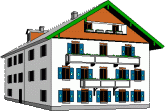
\includegraphics[width=0.4\textwidth]{./inf/SEKII/16_Java_Bilder/haus.png}
\end{center}
